% Created 2019-02-08 ven. 20:43
% Intended LaTeX compiler: pdflatex
\documentclass[11pt]{article}
\usepackage[utf8]{inputenc}
\usepackage[T1]{fontenc}
\usepackage{graphicx}
\usepackage{grffile}
\usepackage{longtable}
\usepackage{wrapfig}
\usepackage{rotating}
\usepackage[normalem]{ulem}
\usepackage{amsmath}
\usepackage{textcomp}
\usepackage{amssymb}
\usepackage{capt-of}
\usepackage{hyperref}
\usepackage{minted}
\usepackage[french]{babel}
\usepackage[x11names]{xcolor}
\hypersetup{linktoc = all, colorlinks = true, urlcolor = DodgerBlue4, citecolor = PaleGreen1, linkcolor = black}
\author{Raoul HATTERER}
\date{\today}
\title{Traitement d'image\\\medskip
\large (1 séance = 1h30)}
\hypersetup{
 pdfauthor={Raoul HATTERER},
 pdftitle={Traitement d'image},
 pdfkeywords={},
 pdfsubject={},
 pdfcreator={Emacs 26.1 (Org mode 9.2)}, 
 pdflang={French}}
\begin{document}

\maketitle
\setcounter{tocdepth}{1}
\tableofcontents




\section{Codage RVB et niveau de gris}
\label{sec:org1b0d0d9}

\begin{itemize}
\item Aller sur \href{https://www.w3schools.com/colors/colors\_rgb.asp}{colors RGB} et tester ce que l'on obtient si l'on remplace chacune des valeurs R, V et B d'un pixel par la moyenne des sous-pixels.
\item Essayer pour plusieurs couleurs.
\end{itemize}


\section{Image de départ}
\label{sec:orgb215a96}

\begin{figure}[htbp]
\centering
\includegraphics[width=.9\linewidth]{pomme.jpg}
\caption{Image de départ}
\end{figure}


\section{Comment lire un pixel}
\label{sec:orgdf47ac8}

Après avoir fait quelques recherches sur ce qu'est un "pixel", voyons comment lire le pixel de coordonnées (100,250).

\begin{minted}[]{python}
from PIL import Image
img = Image.open("pomme.jpg")
r,v,b=img.getpixel((100,250))
print("canal rouge : ",r,"canal vert : ",v,"canal bleu : ",b)
\end{minted}

\begin{verbatim}
('canal rouge : ', 19, 'canal vert : ', 88, 'canal bleu : ', 192)
\end{verbatim}


\section{Comment écrire un pixel}
\label{sec:org43712c9}

\begin{minted}[]{python}
from PIL import Image
img = Image.open("pomme.jpg")
img.putpixel((5,5),(255,0,0))
img.show()
\end{minted}

Question : \emph{Identifier où se trouve l'origine de l'image.}


\section{Que fait le programme suivant ?}
\label{sec:org0fc92f7}

\begin{minted}[]{python}
from PIL import Image
img = Image.open("pomme.jpg")
largeur_image,hauteur_image=img.size
for y in range(hauteur_image):
    for x in range(largeur_image):
        rouge,vert,bleu=img.getpixel((x,y))
        nouveau_rouge=vert
        nouveau_vert=bleu
        nouveau_bleu=rouge
        img.putpixel((x,y),(nouveau_rouge,nouveau_vert,nouveau_bleu))
img.show()
img.save("pommeMystere.jpg")
\end{minted}


On analyse le code ci-dessus qui servira de base pour le défi suivant.

\begin{figure}[htbp]
\centering

\includegraphics[width=.9\linewidth]{pommeMystere.jpg}
\caption{Résultat du programme mystère}
\end{figure}


\section{Passage d'une image en niveaux de gris (codé RVB sur 3 octets)}
\label{sec:org1fde869}

Après avoir fait quelques recherches sur les "images en niveaux de gris", écrivez un programme qui transforme une "image couleur" en une "image en niveaux de gris".

Petite astuce qui pourrait vous aider : en Python pour avoir une division entière (le résultat est un entier), il faut utiliser l'opérateur // à la place de l'opérateur / 

Remarque: On donne l'algorithme aux élèves (ou on le construit avec eux) ; ils doivent alors programmer le passage d'une image couleur à une image en niveaux de gris.


\begin{minted}[]{python}
from PIL import Image
img = Image.open("pomme.jpg")
largeur_image=480
hauteur_image=300
for y in range(hauteur_image):
    for x in range(largeur_image):
       rouge,vert,bleu=img.getpixel((x,y))
       nouveau_rouge=(vert+bleu+rouge)//3
       nouveau_vert=(vert+bleu+rouge)//3
       nouveau_bleu=(vert+bleu+rouge)//3
       img.putpixel((x,y),(nouveau_rouge,nouveau_vert,nouveau_bleu))
img.show()
img.save("pommegrise.jpg")
\end{minted}

\begin{figure}[htbp]
\centering
\includegraphics[width=.9\linewidth]{pommegrise.jpg}
\caption{Pomme Linux en niveaux de gris (codé RVB)}
\end{figure}


\section{Passage d'une image en niveau de gris (luminance codée sur 1 seul octet)}
\label{sec:org23192ac}

\begin{minted}[linenos,firstnumber=1]{python}
from PIL import Image
img = Image.open("pomme.jpg").convert("L")
img.show()
img.save("pommegriseL.jpg")
\end{minted}


\begin{figure}[htbp]
\centering

\includegraphics[width=.9\linewidth]{pommegriseL.jpg}
\caption{Image en niveaux de gris (luminance L)}
\end{figure}

Comparer la taille des différents fichiers. Conclure.


\section{Récréation ou challenge ?}
\label{sec:orgc5abfdc}

\subsection{Créer une image en négatif}
\label{sec:org97f9b16}

\begin{figure}[htbp]
\centering
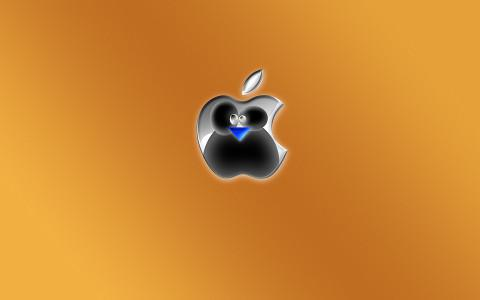
\includegraphics[width=.9\linewidth]{pommeNegatif.jpg}
\caption{Négatif}
\end{figure}

\subsection{Diagonale}
\label{sec:org28b4c9d}

Créer le programme qui garde l'image d'origine au-dessus d'une diagonale et qui transforme en niveaux de gris en-dessous de celle-ci.


\begin{figure}[htbp]
\centering

\includegraphics[width=.9\linewidth]{pommemisgrise.jpg}
\caption{Pomme coupée}
\end{figure}
\end{document}